        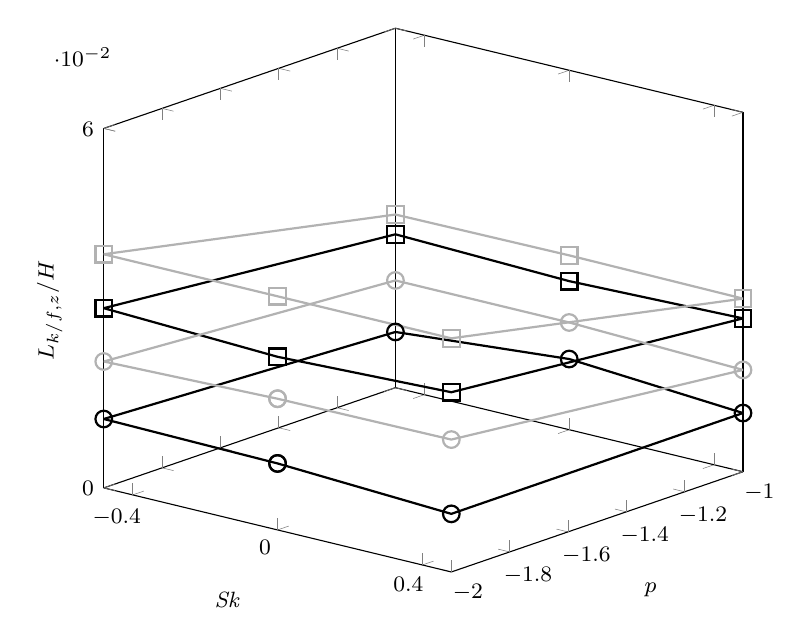
\begin{tikzpicture}[]
        \centering
        \begin{axis}[
        view={40}{20},
            ylabel={$p$},
            xlabel={\textit{Sk}},
			zlabel={$L_{k/f,z}/H$},
			xtick={-0.4,0,0.4},
			ztick={0,0.06},
			zmin=0,zmax=0.06,
            %ymin=0, ymax=0.16,
            width=.8\textwidth,
            height=.7\textwidth,
            label style={font=\footnotesize},
            tick label style={font=\footnotesize}
            ]

            
                                    \addplot3 [
            black,mark=square,thick, mark size=3pt
            ]
            coordinates{
            (0,-2,0.0289)			
			(0.48,-2,0.0300)
			(0.48,-1,0.0256)
			(0,-1,0.0248)
			(-0.48,-1,0.0256)
			(-0.48,-2,0.0300)
            (0,-2,0.0289)
			};
			
			
			\addplot3 [
            gray!60,mark=square,thick, mark size=3pt
            ]
            coordinates{
            
            (0,-2,0.0390)
			(0.48,-2,0.0390)
			(0.48,-1,0.0289)
			(0,-1,0.0291)
			(-0.48,-1,0.0289)
			(-0.48,-2,0.0390)
			(0,-2,0.0390)
            };
            
            
                                                            \addplot3 [
            black,mark=o,thick, mark size=3pt
            ]
            coordinates{
            (0,-2,0.0111)		
			(0.48,-2,0.0097)
			(0.48,-1,0.0098)
			(0,-1,0.0118)
			(-0.48,-1,0.0093)
			(-0.48,-2,0.0115)
            (0,-2,0.0111)
			};
			\addplot3 [
            gray!60,mark=o,thick, mark size=3pt
            ]
            coordinates{
            (0,-2,0.0219)
			(0.48,-2,0.0221)
			(0.48,-1,0.0170)
			(0,-1,0.0179)
			(-0.48,-1,0.0179)
			(-0.48,-2,0.0211)
			(0,-2,0.0219)
            };
            
            
        \end{axis}
        \end{tikzpicture}